\section{Virtual Memory}

From previous courses we know MMUs, TLBs and basic paged virtual memory operations. The uses for address translation include:
\begin{itemize}
	\item Process Isolation
	\item Shared Code Segments
	\item Dynamic Memory Allocation
	\item Persistent Data Structures
	\item etc.
\end{itemize}

\subsection{Segments}

Before paging, there were segments. Before segments there where base and limit registers. These contained two addresses $B$ and $L$. A CPU access to an address $a$ is permitted iff $B \leq a < L$. Relocation registers are an enhanced form of base register. All CPU accesses are relocated by adding the offset: a CPU access to an address $a$ is translated to $B + a$. This allows each program to be compiled to run at the same address (e.g. 0x0000). \medskip
\begin{center}
	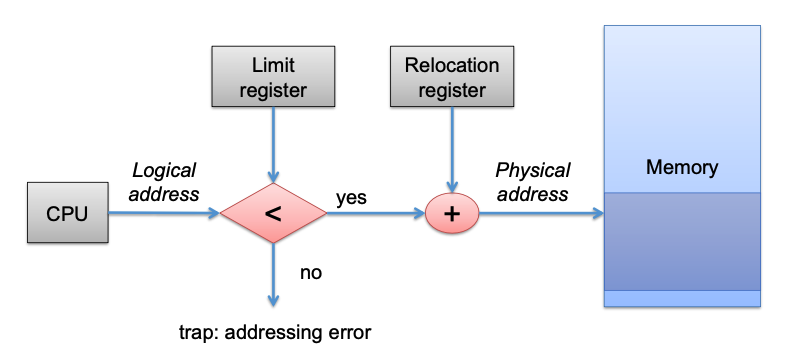
\includegraphics[width=\linewidth]{base-relocation-register.png}
\end{center}

A segment is a triple $(I, B_I, L_I)$ of values specifying a contiguous region of memory address space with base $B_I$, limit $L_I$, and an associated segment identifier $I$ which names the segment. Memory in a segmented system uses a form of logical addressing: each address is a pair $(I, O)$ of segment identifier and offset. A Segment Table is an in-memory array of base and limit values $(B_I, L_I)$ indexed by segment identifier, and possibly with additional protection information.
\begin{center}
	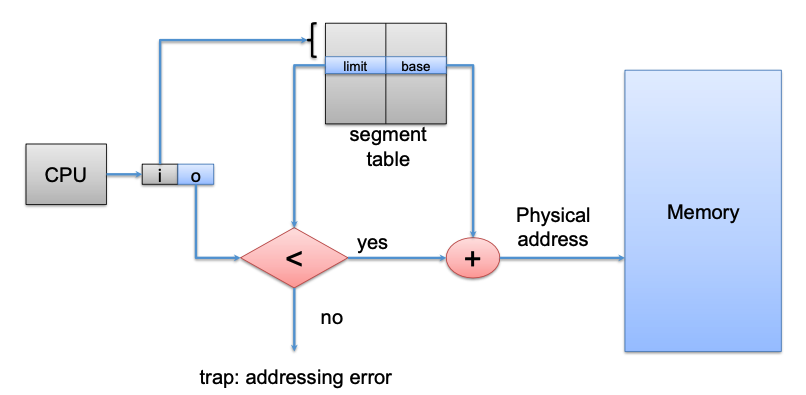
\includegraphics[width=\linewidth]{segment.png}
\end{center}

This enables sharing code/data segments between processes, further it adds protection and allows transparently growing stack/heap as needed. The principal downside of segmentation is that segments are still contiguous in physical memory, which leads to external fragmentation.

\subsection{Paging}

This is a short recap of paging. Virtual memory is divided into (virtual) pages of the same size having a VPN, physical memory gets divided into frames / physical pages having a PFN / PPN. Then a page table gets used to map VPNs to PFNs. This is implemented in hardware as the MMU. To speed up translation the TLB is used. Getting data from memory can work as follows (in this case we have a TLB miss):
\begin{center}
	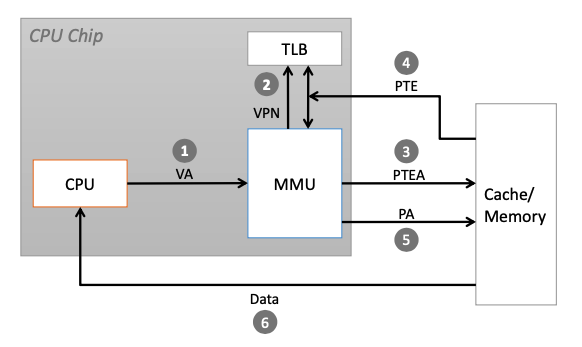
\includegraphics[width=\linewidth]{tlb-miss.png}
\end{center}

We have also seen how multi-level page tables work. Multi-level translation allows us to allocate only page table entries that are in use and makes memory allocation simpler.
\begin{center}
	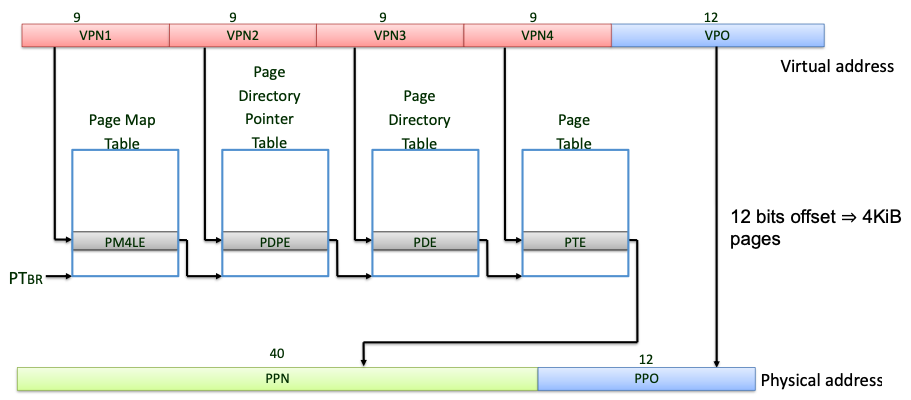
\includegraphics[width=\linewidth]{multi-level-pt.png}
\end{center}

On a context switch we need to store/restore the pointer to the page table and its size. One of the downsides of paging is if our page is very small and we do not need all of the space, this leads to internal fragmentation.

\subsection{Paged Segmentation}

It is possible to combine segmentation and paging. A paged segmentation memory management scheme is one where memory is addressed by a pair (segment.id, offset), as in a segmentation scheme, but each segment is itself composed of fixed-size pages whose page numbers are then translated to physical page numbers by a paged MMU.
\begin{center}
	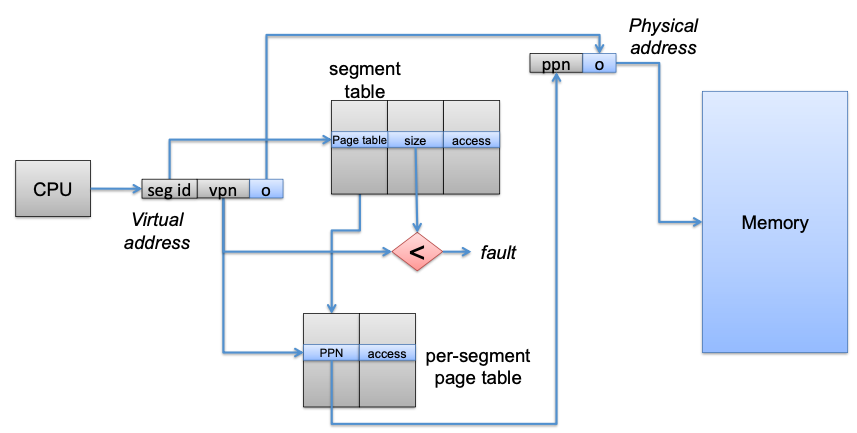
\includegraphics[width=\linewidth]{paged-segments.png}
\end{center}

One of the main benefits here is that each segment can have its own size of page table.

